\chapter{Side Channels}
At any given moment, in the system informations are constantly flowing, because
it is an intrinsic phenomenon of computation. This is true both for a single computer system and a
distributed one.\\
Anyway, all those information flows use intended, specific and implemented channels, in which the
data requires some security guarantees, such as integrity, availability, non-repudiation, \dots\\
Keep in mind that the hardware in consideration have been already verified  and is implementing all
the security and reliability measures that are required.
\begin{section}{Covert Channels}
  \begin{boxH}
    A covert channel is a path for an illegal flow of information within a system.
  \end{boxH}
  Any communication channel that a process can exploit to transfer information in a manner that
  violates the system’s security policy.

  There are many types of covert channels within a computing system, based on what the covert channel
  actually is:
  \begin{itemize}
    \item Timing covert channels
    \item Termination covert channels(eg: it a computation terminates)
    \item Probability covert channels
    \item Resource utilization covert channels
    \item Power covert channels
  \end{itemize}

  One nasty thing about covert channel is the fact that they exploit the functional behaviour of the
  system itself, by just observing its behaviour, in particular differences in scenarios, to
  retreive some data.\\
  For example one could observe the time needed to carry out an encryption operation, and by
  noticing that some particular algorithm need more time for longer keys, it is possible to 
  tell how long the key is, which can make a brute force attack easier. Of course, this is a
  simple example, but it is possible to carry out more complex attacks to retrieve more data.\\

  There are many uses of covert channels to both improve and undermine the security of a computing
  system:
  \begin{itemize}
    \item Exfiltrate data from an otherwise secure system
    \item Avoid detection of unauthorized access
    \item Install, spread, or control malware on compromised systems
    \item Circumvent content or resource filters
    \item Bypass firewalls for unrestricted access
    \item Malware authors use timing to detect analysis sandboxes
  \end{itemize}

  But most importantly, every covert channel provides a \textbf{bandwidth}, which is the amount of
  information that can be transmitted through the channel in a certain amount of time, and a
  \textbf{noise}, which is the amount of distortion that the channel introduces in the data.\\
  This is important both from the point of view of the attacker and the defender: from the attacker
  point of view, he'd like to choose, because covert channels are unavoidable, the channel with the
  highest bandwidth and the lowest noise, while from the defender point of view, he can influence
  those two aspects to make the channel less effective.\\

  It is usually infeasible for realistic systems to eliminate every potential covert
  channel, so some usable techniques against them are to inject noise in the channel or monitor the
  pattern used to exploit the channel.
\end{section}

\begin{section}{Side Channels}
  Side channels are most flexible, because they can be used for a large variety of uses, both to
  improve or undermine the security of a system.\\
  \begin{boxH}
    A side channel is an \textbf{unintended conduit} to \textbf{gain information} about the state or
    operation of the computing system.
  \end{boxH}
  Every side channel have some defining characteristics:
  \begin{itemize}
    \item the existent, or if the channel is a potential one
    \item the bandwidth of the channel, or how much information can be transmitted
    \item how noisy it is, because informations can be distorted or lost by it
  \end{itemize}
  A \textbf{side channel attack} is an attacks based on the analysis and exploitation of side channel
  information. The basic of all this kinds of attacks is the fact that a lot of the resources on a
  computer, and in particular a microprocessor, are shared, and because of this, it is possible to
  observe them, and manipulate them to set their state in a particular way.\\

  \begin{subsection}{Timing Attacks}
    \begin{boxH}
      A timing side-channel attack tries to recover sensible data by \textbf{measuring computation
      time} in a hardware device.
    \end{boxH}
    The timing of a computation can be influenced by many factors, like the cache state, the branch 
    predictor, the memory state, and many others, and by simply observing the time needed to carry
    out a computation, it is possible to retrieve some data.\\
    Let's consider the code snippet, which is a portion of the RSA algorithm:
    \begin{minted}{c}
      Z = 1;
      for i=j-1 downto 0 {
        Z = Z * Z mod N //Square
        if (k[i]==1) {
          Z = Z * X mod N //Multiply
        }
      }
    \end{minted}
    It highlights how the multiplication is not necessary if the bit is 0, but because if the
    conditional operation is carried out, the previous one is basically executed two times(notice
    that they are equal), and the data is surely in the cache, at least after the first iteration,
    i'm able to tell if the bit is 1 or 0, because the operation is taking twice as long, and thus
    retrieve the key.\\
    If you are wondering how one can tell how to observe the execution time with such a small
    granularity, the answer lies in the fact that the instructions are, at least in this case,
    parsed in assembly, which means that a for loop is just a conditional jump. This means that
    after the jump instruction i can most likely observe a small delay before the next instruction,
    and this concept is used also to tell if the conditional operation is executed or not.\\
  \end{subsection}

  \begin{subsection}{Power attacks}
    Power based side channel attacks work in a similar fashion to timing attacks, but instead of 
    profiling the time needed to carry out a computation, they \textbf{profile} the \textbf{power 
    consumption} of the device.\\
    There are two approaches to this kind of attacks, depending on the purpose of the attack, but
    all the devices have two power components:
    \begin{itemize}
      \item the static power, or the amount of power that is consumed to make everything work
      \item the dynamic power, or the amount of power that is consumed to carry out a computation
    \end{itemize}
    We observe the latter one.
    \begin{subsubsection}{Simple Power Analysis}
      Simple Power Analysis (SPA) is a technique that uses the power consumption of a device over a
      period of time to extract information about the data being processed.\\
      Since different operations will exhibit different power profiles, one can determine what type
      of function is being performed at a given time.\\
      Let's take a look at the same snippet of code from the RSA algorithm as before. It is possible
      to notice that if the conditional operation is executed, the power consumption will be higher
      than if it is not, because the multiplication operation is carried out. This is shown in
      figure \ref{fig:power attack}.\\
      \begin{figure}[h]
        \centering
        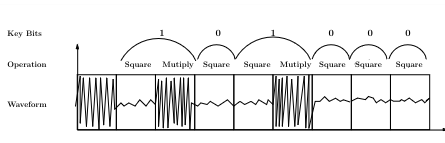
\includegraphics[width=0.5\textwidth]{img/hardware/power attack.png}
        \caption{An example of a SPA attack}
        \label{fig:power attack}
      \end{figure}
      Simple power attacks is quite easy to carry out, but its not always suitable for a power
      attack, because the power profile can be influenced by many factors, like the interrupts or
      the presence of pheripherals, and because we don't know exactly whats going on, it is hard to
      tell what is the cause of the power consumption.
    \end{subsubsection}
    \begin{subsubsection}{Differential Power Analysis}
      \begin{boxH}
        Differential Power Analysis (DPA) is a statistical method for analyzing power consumption to
        identify data-dependent correlations.
      \end{boxH}
      It takes multiple traces (which requires more time and energy to collect) of two data sets and
      try to spot correlations between them.\\
      This is done by computing the average difference of these traces. If the difference is close
      to zero, the two sets are not correlated, otherwise they are.\\
      Given enough traces, even tiny correlations can be seen, regardless of how much noise is in
      the system, since the noise will effectively cancel out during the averaging. This means that
      out of a large number of traces, the noise will be averaged out, while the signal will remain
      and be visible.

      \begin{figure}[h]
        \centering
        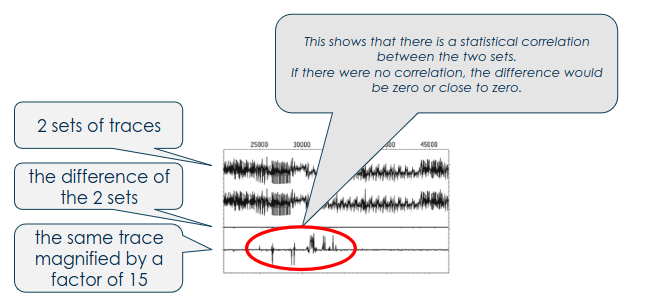
\includegraphics[width=0.7\textwidth]{img/hardware/dpa attack.png}
        \caption{An example of a DPA attack}
      \end{figure}
      Furthermore, this kind of attack has some benefits, in fact, even if they require some
      knowledge of the running algorithm (the physical implementation is not required), they are
      quite cheap to perform, because they need only to perform the measurements and correlate the
      power consumption of the device and the encryption data, including the key.\\
    \end{subsubsection}

  \end{subsection}

\end{section}

\begin{section}{Cache attacks}
  Cache attacks are one of the most powerful, and used one, to create a side channel to exploit some
  other observations and bugs. They are based on the fact that cache are all about reducing latency
  of consecutive memory access, and because they are, mostly(eg: L1 caches), shared resources, it is
  possible to observe its state even if its not possible to directly address their memory, just by
  observing temporal differences in memory access.\\
  Many attacks uses the cache as a covert channel, like meltdown, spectre(meltdown v3), LVI(meltdown
  v4), mds(ridl/zombieload), branchscope, and many others.\\
  Different attacks exploits different features of caches, which, for the most part are:
  \begin{itemize}
    \item the cache is a shared resource
    \item the cache latency in case of miss and hit
    \item the cache associativity
    \item the cache replacement policy
  \end{itemize}
  For example the spectre attack exploits the fact that during the microarchitectural execution no
  memory boundaries are checked, in particular memory that has the same privileges, the privesc part
  is a feature of MeltdownUS/v1, and by achieving a particular memory configuration in the cache, it
  is possible to start the execution of instructions that would never be executed otherwise, because
  some required data is not available, being flushed beforehand. Than by measuring the latency of
  consecutive memory access, it is possible to retrieve the accessed data by iterating the same
  process over and over again.

\end{section}

\begin{section}{Cloud/FPGA Side-Channel}
  The FPGA boards can be exploited to create a covert channel, in particular the thermal and power
  to retrieve some data from the system.\\
  For example, by observing the temperature of a threshold of the FPGA, it is understand if the data
  that is being processed is a 1 or a 0, because the power consumption of the FPGA is different
  based on the data that is being processed.
\end{section}

\begin{section}{Side channel defenses}
  Removing a side channen, as already stated, is not always possible, because it involves some
  changes on the hardware, as well as trying to preventing them. The second second solution is to
  make the channel less effective. There are many approaches to defend against side channels, but
  the most effective one is to inject some noise in the channel. This is because a side channel, to
  be effective needs accurate measurements to retrieve some data, and by injecting noise in the
  channel, the measurements will be distorted, and the data will be harder to retrieve.\\
  Other approaches are:
  \begin{itemize}
    \item Leakage Reduction
    \item Key Update
    \item Side channel-resistant PUFs
    \item Secure scan chains
  \end{itemize}
  \begin{subsection}{Countermeasures against DPA}
    One of the most common is the introduction of random process interrupts. Instead of executing
    all the operations sequentially, the CPU interleaves the code’s execution with that of dummy
    instructions so that corresponding operation cycles do not match because of time shifts. The
    introduction of dummy instructions smears the peaks across the differential trace due to a
    desynchronization effect, known in digital signal processing as incoherent averaging.
  \end{subsection}

  \begin{subsection}{Process isolation}
    Another approach is to use process isolation techniques, like enclaves, to isolate the
    execution of a process, at the cost of hardware utilization. After all, there's no actual
    implementation that supports multi-core systems to secure the computation.
  \end{subsection}

  \begin{subsection}{Janus Cache}
    Another approach to deal with side channel is to change the behaviour of some components, like
    the cache, in a way that doesn't change the outcome of the computation, but makes life harder
    for the attacker, eg: by introducing some delay on purpose.\\
    This is the basic idea of the Janus cache. One bit is added to the cache, the \textit{ON\_OFF flag}
    , which is used to determine the behaviour of the cache line. If the flag is set, even if
    the data is in the cache, the cache line cannot be accessed, functionally introducing a delay,
    because the data must be fetched from the memory.\\

    \begin{figure}[h]
      \centering
      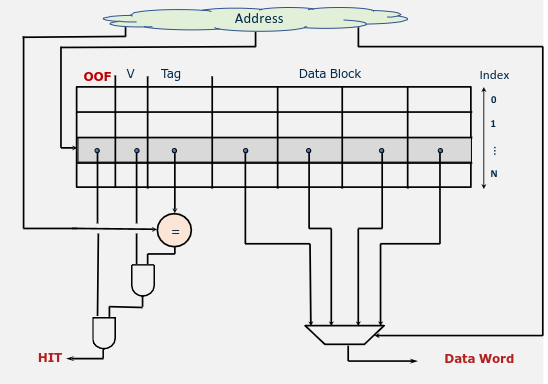
\includegraphics[width=0.5\textwidth]{img/hardware/janus cache.png}
      \caption{An example of a Janus cache}
    \end{figure}

  \end{subsection}

\end{section}

